\subsection{Deeper Granular Refinement}
\label{sec:granularityFRESHAlg}
%Model elements considered for the \aivcalg algorithm are explicitly defined in the Lustre code -- these we call \emph{IVC elements}; the generation of Lustre from an AADL/AGREE model provides guarantees and assumptions as IVC elements and when fault analysis is run using the safety annex, constrained faults are also added to this set. This can be seen in the safety analysis modified Lustre code in Figure~\ref{fig:lustreSensorsSafety} which is nominally the same as Figure~\ref{fig:lustreSensors}, but has faulty information added to outputs and IVC elements\footnote{For more information on safety modified Lustre programs, see Chapter XX, Section XX \danielle{ADD THIS TO IMPL}}. 

%\danielle{Add figure of lustre code. Highlight IVC elements.}

As previously described, we explored granularity within the context of the Lustre language; this programming language provides a good formalism for discussion because it is top-level conjunctive, equational, and \emph{referentially transparent}: the behavior or a Lustre program is defined by a system of equations, and any subexpression on the right side of an equation can be extracted and assigned to a fresh variable which is substituted into the original equation without changing the meaning of a program~\cite{Halbwachs91:IEEE,ghassabani_2018}. In this context, we can define a \emph{granular refinement} as an extraction of a subexpression into a new equation assigning a new variable. 

The maximal factorization of the model can be obtained by assigning each instance of a subexpression and each use of an input to its own variable. This results in a \emph{totally decomposed} Lustre model: (1) each computed (non-input) variable is used at most once in the right side of an equation, (2) each equation is either a single operator or a constant expression, and (3) each model input is directly assigned to one or more fresh variables and is not used elsewhere in the model~\cite{ghassabani_2018}.

Ghassabani performed a preliminary analysis on maximally factored models for IVC coverage and found that analysis performed significantly slower for proofs and the \ivcmust algorithm. For our purposes in safety analysis, our concern is the guarantees in the Lustre model; therefore, we are able to weaken the factorization performed. To this end, a \emph{partially decomposed} Lustre model has the properties that (1) each computed variable is used at most once in the right side of an equation, and (2) each guarantee and associated equation has either a single operator or a constant expression. 










\begin{comment}
Model elements considered for the \aivcalg algorithm can be explicitly defined in the Lustre code -- these we call \emph{IVC elements}; the generation of Lustre from an AADL/AGREE model provides guarantees and assumptions as IVC elements and when fault analysis is run using the safety annex, constrained faults are also added to this set\footnote{For more information on safety modified Lustre programs, see Section~\ref{sec:impl}}.  The \aivcalg algorithm also contains an option to assign all equations in the model as IVC elements. 


For the purposes of fault analysis and minimal cut set generation, we performed a partial decomposition of the contracts on the guarantees of the model in Lustre. An example of the simplified Lustre code before and after decomposition is shown in Figure~\ref{fig:lustreTwoGuar} and Figure~\ref{fig:lustreDecompGuar}. \danielle{change this to lustre direct fresh vars}

\begin{figure}[h!]
\begin{center}
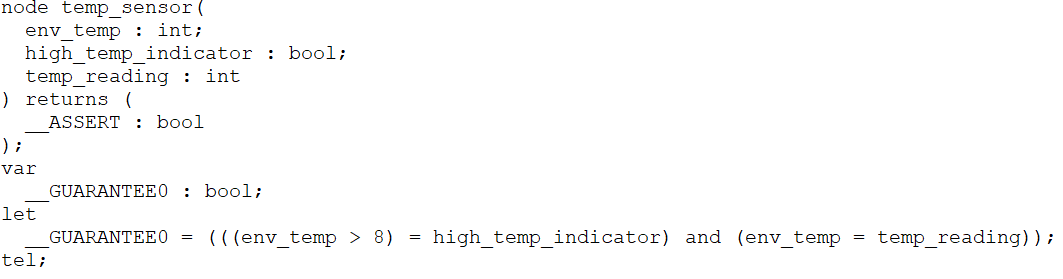
\includegraphics[width=.9\textwidth]{images/lustreTwoGuar.PNG}
\caption{Temp Sensor With Original Guarantee} \label{fig:lustreOneGuar}
\end{center}
\end{figure} 

\begin{figure}[h!]
\begin{center}
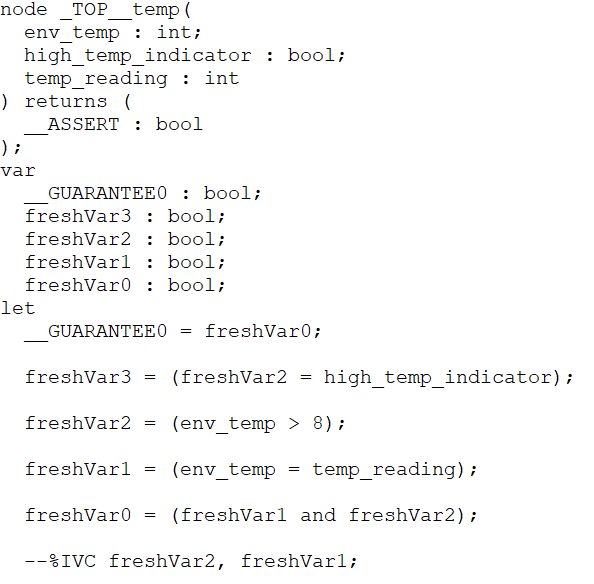
\includegraphics[width=.7\textwidth]{images/lustreDecomposedGuarantee.PNG}
\caption{Temp Sensor With Decomposed Guarantee} \label{fig:lustreDecompGuar}
\end{center}
\end{figure} 

The initial guarantee of interest -- \texttt{GUARANTEE0} from Figure~\ref{fig:lustreOneGuar} -- is decomposed and broken down into a series of fresh variables, \texttt{freshVar0} through \texttt{freshVar3} as seen in Figure~\ref{fig:lustreDecompGuar}. The fresh variables are then added to the IVC elements to put them into scope for the \aivcalg algorithm. The partial decomposition of the guarantees was performed according to Algorithm~\ref{alg:decomp}. \danielle{Rewrite algorithm.}

\begin{algorithm}[h]
\DontPrintSemicolon
\SetKwFunction{Init}{Init}
\SetKwFunction{Decompose}{Decompose}
\SetKwProg{Fn}{Function}{:}{}
\Fn{\Init{$G$}}{
	$G$:= guarantee in Lustre node \;
	$\mathit{newLocalVars} \gets \emptyset$
	$\mathit{freshVar} \gets \mathit{g.expr}$ \;
	$\mathit{newGuar} \gets \mathit{freshVar}$ \;	
	$\mathit{newLocalVars} \gets \mathit{\Decompose(g.expr)}$ \;
	
}

\setcounter{AlgoLine}{0}
\Fn{\Decompose{$\mathit{expr}$}}{
	$\mathit{freshVars} \gets \emptyset$ \;
	\eIf{$\mathit{expr}$ is constant $\lor$ has single operator}{
		\textbf{return} $\mathit{freshVars}$
	}{
		$\mathit{freshL} \gets \mathit{expr.left}$ \;
		$\mathit{freshR} \gets \mathit{expr.right}$ \;
		$\mathit{freshVars.add(\{freshL, freshR\})}$ \;
		$\mathit{\Decompose(expr.left)}$ \;
		$\mathit{\Decompose(expr.right)}$ \;
	}
}
	\caption{Decomposition of Guarantees}
	\label{alg:decomp}
\end{algorithm}

The AGREE program is intercepted by the safety annex plugin as described in Section~\ref{sec:impl}. Each guarantee defined in the nodes are decomposed and fresh variables are added to the local variables and their assignment added to local equations. This modified program is returned to AGREE along with the fault model modifications and the MIVCs are computed. As usual, the minimal cut sets are found according to the MIVC results. 

\end{comment}







We were interested in three main research questions regarding the exploration of granularity refinement: 

\begin{description}
\item [RQ1:] What is the analysis time difference between the nominal model MIVC generation and the decomposed model MIVC generation? Given smaller models with fewer or less complex guarantees, the timing results should not differ greatly, but in a large model with potentially many complex guarantees, the computation time for MIVC generation could increase quickly. 

\item[RQ2:] Do the MIVCs generated reflect a more accurate view of which portions of the model support the proof of the safety property? We expect that the additional granularity would provide more exact coverage of the model in terms of the MIVCs. 

\item[RQ3:] Given the results in RQ2, could more exact minimal cut sets be produced from the MIVCs? If changes are reflected in the MIVC sets, then we will see corresponding changes in the minimal cut sets. This could provide more exact safety analysis artifacts and additional insight into the specifications and how they impact the analysis results. 
\end{description}

To address these questions, we developed an algorithm that performs a partial decomposition of the equations in the Lustre model. For our purposes in safety analysis and minimal cut set generation, the equations that will be of interest are the guarantees in the nominal model and any associated equations; therefore, we perform the refactorization on equations alone. 

The logical structure of a formula can be viewed as a tree where nodes are arranged in terms of operator precedence. Clearly, it is a requirement to preserve equivalence during refactoring and we do not want to change the semantics of the formula, only the structure. To this end, we isolated branches and subtrees of the structure so that the \aivcalg algorithm can view each subtree of the formula separately. The algorithm we use recursively travels down a formula tree, assigning each subtree as a fresh variable. Figure~\ref{fig:formulaTree} shows the following formula in tree form where \textit{lit} refers to a literal and \textit{const} refers to a constant:
\begin{gather*}
((((\mathit{const} \implies \mathit{lit}) \lor \mathit{const}) \iff \mathit{lit} ) \land (\mathit{lit}  \lor \mathit{lit} )) 
\end{gather*} 

\begin{figure}
\begin{center}
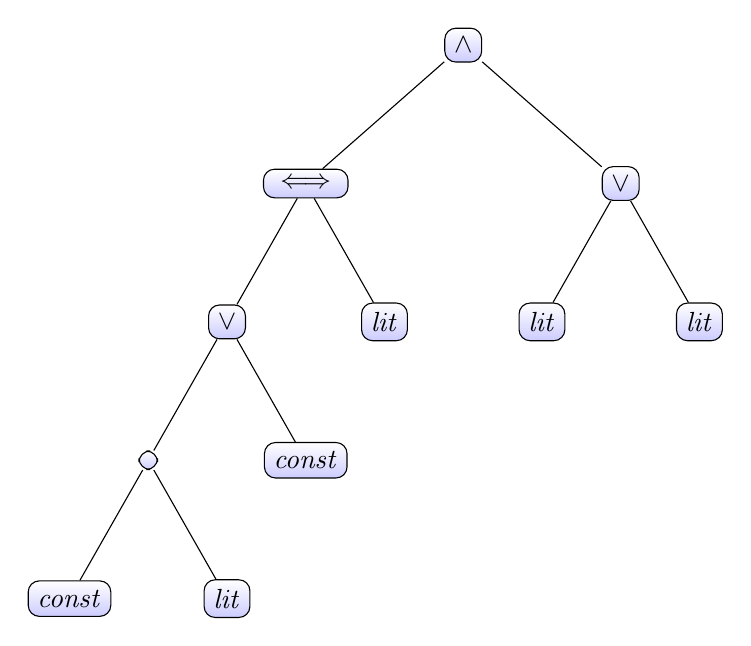
\begin{tikzpicture}[level distance = 5em, every node/.style = {shape=rectangle, rounded corners,
    draw, align=center,
    top color=white, bottom color=blue!20}]]
  \tikzstyle{level 1}=[sibling distance=40mm] 
  \tikzstyle{level 2}=[sibling distance=20mm] 
  \tikzstyle{level 3}=[sibling distance=20mm] 
\node {$\land$} 
    child { node {$\iff$} 
	  child{ node{$\lor$}  
 	    child{node{$\implies$} 
            	 child{ node{\textit{const}}  } 
	          child{ node{\textit{lit}}  }   
 	    }
 	    child{node{\textit{const}}}	  
	  }
	  child{ node{\textit{lit}}  }    
    }
    child { node {$\lor$}
      child { node {\textit{lit}} }
      child { node {\textit{lit}} } } ;
\end{tikzpicture}
\end{center}
\caption{Graphical Representation of a Boolean Formula}
\label{fig:formulaTree}
\end{figure}

As seen in Figure~\ref{fig:formulaTree}, the leaf nodes of the tree are constants and literals; these are the base cases in the recursion. Each square node represents a subformula and is a recursive case. The refactored equation is shown in Figure~\ref{}. Each subformula is assigned a fresh variable and added to the equations for the Lustre node. The fresh variables are also assigned to be IVC elements and considered during the \aivcalg algorithm. 

%Each equation in the Lustre model is refined as shown in Figure~\ref{}. \danielle{show original lustre equation and the refactored equation.} By assigning fresh variables recursively throughout the equations, it allows the MIVC algorithm a deeper insight into the coverage of each piece of the original equation itself. As an example, we look at \danielle{}

%Model elements considered for the \aivcalg algorithm can be explicitly defined or the algorithm can take into consideration all equations, inputs, and variables in a program by use of the \texttt{--all-assigned} flag in JKind. In this implementation, we use the \texttt{--all-assigned} parameter on decomposed equations in each node of a Lustre model.